\section{Motivation}\label{sec:motivation_md_2022}
As discussed in the previous chapter, PyHEADTAIL simulations including the SPS impedance model suggest that the beam coupling impedance leads to an effective suppression of the $\CC$ RF phase noise induced emittance growth through the separation of the coherent tune from the incoherent spectrum. This suppression, which is related to the coherent (dipole) motion, can reach up to a factor of 4-5 for the experimental conditions of the first experimental campaign with $\CC$s that took place in the SPS in 2018, which seems to be the explanation for the experimental observations (see Section~\ref{sec:MD5_overview}).

This suppression effect has never been observed before. To this end, another experimental campaign took place in the SPS in 2022 where the main objective was to validate experimentally the above-mentioned suggested emittance growth suppression mechanism. If successful, it would constitute the first experimental investigation and validation of this effect. Moreover, achieving a good understanding of the 2018 results is essential for developing confidence in the theoretical model and its predictions for the HL-LHC.

The experimental campaign of 2022, was organised in two proof-of-concept experiments. The first experiment was carried out in the presence of phase noise in the $\CC$ RF system. The second experiment took place with a pure dipolar noise source: the beam transverse damper. This chapter reports on the preparation, the methodology, and the results of these experiments.

\section{Experiment with CC as noise source}\label{sec:cc_md_2022}
Due to the preceding PyHEADTAIL simulations which provided strong evidence that the observed discrepancy between the 2018 measurements and the theoretical predictions could be explained by the beam transverse impedance additional machine time was dedicated to emittance growth studies with $\CC$ in the SPS in 2022. The time allocated for the $\CC$ experiment was limited to about 10 hours since many different studies have to take place in the SPS during the year. Taking into consideration the time needed for the setup and the $\CC$ calibration the time available for the emittance growth measurements is reduced even more. To this end, measurement repeatability is limited and the experimental procedure had to be carefully planned in advance.
% Also you can add that each point in the emittance growth studies needs about 30-40 min.

\subsection{Machine and beam configuration}\label{sec:cc_md_2022_parameters}
The emittance growth measurements in 2022 were performed in coast at 270\,GeV following the same setup as in 2018 (see Section~\ref{sec:exp_setup_2018}) and very similar machine and beam conditions. The most relevant ones are listed in Table~\ref{tab:machine_beam_param_2022}. 

The linear chromaticity was corrected to about zero units in both the horizontal and vertical planes. That was a result of miscommunication with the operator team of the SPS machine as the desired value was between 0.5 and 1.0. However, the analysis of the PyHEADTAIL simulations in Section~\ref{subsec:chroma_scan} showed that the sensitivity of the emittance growth suppression to the linear chromaticity values (for small positive values) is expected to be insignificant. 

On the grounds that the last three (out of four) bunches used in 2018 expereimental campain were unstable, in 2022 the experiment was carried out with a single bunch. This choice allowed also to have better control on the beam conditions, avoiding possible effects from interactions within the bunches \footnote{Even though these effects should be insignificant due to the large bunch spacing, see Table~\ref{tab:machine_beam_param_2018}.}.

\begin{table}[!hbt]
	\begin{minipage}{\textwidth}
      \begin{centering}
   \caption{Main machine and beam parameters for the emittance growth studies with CCs in SPS in 2022.}
	\begin{tabu} to \textwidth {X[c,m] X[0.5c,m] X[0.5c,m] X[0.01c,m]}
		&&& \\[-6mm]
		\toprule \toprule
		\multicolumn{2}{l}{\textbf{Parameter}} &
		\multicolumn{2}{c}{\textbf{Value}} \\
		\bottomrule
      \multicolumn{2}{l}{Beam energy, $\symE$} & \multicolumn{2}{c}{270\,GeV} \\
      \multicolumn{2}{l}{Main RF voltage / frequency,  $\VRF$ / $\fRF$}  & \multicolumn{2}{c}{5\,MV / 200.39\,MHz} \\ %200.3945
      \multicolumn{2}{l}{Horizontal / Vertical betatron tune, $\Qx$ / $\Qy$}  & \multicolumn{2}{c}{26.13 / 26.18} \\
      \multicolumn{2}{l}{Horizontal / Vertical first order chromaticity, $\Qpx$ / $\Qpy$}  & \multicolumn{2}{c}{ $\sim$ 0.0-0.5 / $\sim$ 0.0-0.5} \\
      \multicolumn{2}{l}{Synchrotron tune, $\Qs$}  & \multicolumn{2}{c}{0.0051} \\
      \multicolumn{2}{l}{$\CC 1$ voltage / frequency, $\VCC$ / $\fCC$}  & \multicolumn{2}{c}{1\,MV / 400.78\,MHz} \\
      \multicolumn{2}{l}{Number of protons per bunch, $\Nb$} & \multicolumn{2}{c}{3 $\times 10^{10}$ p/b$^\ast$} \\
      \multicolumn{2}{l}{Number of bunches}  & \multicolumn{2}{c}{1} \\
      \multicolumn{2}{l}{Rms bunch length, 4$\sigmat$}  & \multicolumn{2}{c}{1.83 \,ns$^\ast$}\\
      \multicolumn{2}{l}{Horizontal / Vertical normalised emittance, $\emitx$ / $\emity$}  & \multicolumn{2}{c}{2\,$\mathrm{\mu m}$ / 2\,$\mathrm{\mu m^\dagger}$}\\
      \multicolumn{2}{l}{Horizontal / Vertical rms tune spread, $\Dqxrms$ / $\Dqyrms$}  & \multicolumn{2}{c}{2.02 $\times 10^{-5}$ / 2.17 $\times 10^{-5}$ $^\ddagger$}\\
      \bottomrule
	\end{tabu}
   \label{tab:machine_beam_param_2022}
   \end{centering} \footnotesize{$^\ast$ This value corresponds to the average r,s measured bunch length over all the coasts of 2022.\\$^\dagger$ The value corresponds to the requested intial value at the start of each coast. Nevertheless, the intensity drop and the bunch length increase were found to be insnificant for all the coasts. \\$^\ddagger$ Here the rms betatron tune spread includes only the contribution from the detuning with amplitude present in the SPS machine. More details along with the calulcations for the listed values can be found in Appendix~\ref{app:detuning_with_amplitude}.}
   \end{minipage}
\end{table}
% For bunch length: cernbox/2022/SPS_MDs_2022/cc_md_16May2022/longitudinal_profiles/visualise_pickle.ipynb

The average rms bunch length (over all settings) was measured to be about $4\sigma_t$ = 1.83\,ns. During the coasts, an increase of $\sim$5~$\%/h$ on average for each setting was observed. This small increase agrees with what is usually observed in the SPS in coast and will not be taken into consideration in the following analysis. The individual plots illustrating the evolution of the bunch length as measured by the ABWLM during the experiment can be found in the Appendix..... Last, looking at the dependence of the emittance growth suppression by the impedance on the bunch length in Fig.~\ref{fig:study_10_bunch_length} it is evident that the rms bunch length of $4\sigma_t$ = 1.83\,ns belongs to the regime of the strong suppression optimizing the experimental conditions to observe the impedance effects on the noise-induced emittance growth.

The intnesity was set to $3 \times 10^{10}$ protons to be in agreement with the experiment of 2018. During the coasts of the 2022 experiment almost zero losses were observed. Therefore, the evolution of the intensity during the coasts will be not considered in the following.


\textbf{CC RF noise}\\
The noise injected in the $\CC$ RF system was again a mixture of phase and amplitude noise. The noise excitation extended from DC up to 10\,kHz and thus the noise was applied on the first betatron sideband only, at $\sim$8\,kHz. The PSD values at $\sim$8\,kHz of the four different levels of artificial noise that were used in the experiment are listed in Table~\ref{tab:noise_settings_2022}. By looking at the table, it becomes evident that the contribution of amplitude noise to the total emittance growth was found to be insignificant (about 7$\%$). To this end, in the post-processing of the 2022 data, the introduction of the effective phase noise (see Section~\ref{sec:injected_RF_noise}) is not required. In the following, the measured growth rates will be displayed as a function of the measured RF phase noise only. This choice is also justified by the fact the objective of the 2022 experimental campaign with $\CC$s is to mainly reproduce the qualitative expected bahevior from the impedance and not the exact values. This is discussed further in the next sections of this chapter.

% I don't have the data to plot the spectra. Only screenshots in the logbook.


% Note 1: Noise level values from the logbook.
% Note 2: Analysis and percentages: /2022/SPS_MDs_2022/cc_md_16May2022/roundA_online_analysis_ws/summary_plots/for_thesis/cc_md_analysis_noise_scan_for_thesis.ipynb
\begin{table}[!hbt]
	\centering
   \caption{Phase and amplitude noise levels injected in the CC RF system for the emittance growth studies of 2022 along with the analytically expected growths. The listed noise values correspond to the PSD values at the first betatron sideband, $f_b$, at $\sim$8\,kHz. The analytical emittance growth rates were computed using Eq.~\eqref{eq:dey_an} and~\eqref{eq:dy_pn} for rms bunch length of $4\sigma_t$=1.83\,ns.}
	\begin{tabu} to \textwidth { X[c,m] X[c,m] X[c,m] X[c,m] X[c,m]}
		&&&& \\[-6mm]
		\toprule \toprule
		\multicolumn{1}{l}{} &
		\multicolumn{2}{c}{$\mathbf{10\,\boldsymbol{\log}_{10} \mathcal{L}(f)}$ \textbf{[dBc/Hz]}} & \multicolumn{2}{c}{\textbf{Analytical } $\mathbf{d \boldsymbol{\epsilon}_y/dt \ [\boldsymbol{\mu} m/h]}$} \\
		\bottomrule
      \multicolumn{1}{l}{} & 	\multicolumn{1}{c}{\textbf{Phase noise}} & \multicolumn{1}{c}{\textbf{Amplitude noise}} & \multicolumn{1}{c}{\textbf{Phase noise}} & \multicolumn{1}{c}{\textbf{Amplitude noise}} \\
      \midrule
      \multicolumn{1}{l}{Level 1}  & \multicolumn{1}{c}{-115.2} & \multicolumn{1}{c}{-124.6} & \multicolumn{1}{c}{1.64} & \multicolumn{1}{c}{0.16} \\
      
      \multicolumn{1}{l}{Level 2}  & \multicolumn{1}{c}{-109.5} & \multicolumn{1}{c}{-120.5} & \multicolumn{1}{c}{6.11} & \multicolumn{1}{c}{0.42}\\

      \multicolumn{1}{l}{Level 3}  & \multicolumn{1}{c}{-104.7} & \multicolumn{1}{c}{-116.0} & \multicolumn{1}{c}{18.44} & \multicolumn{1}{c}{1.19} \\

      \multicolumn{1}{l}{Level 4}  & \multicolumn{1}{c}{-100.1} & \multicolumn{1}{c}{-111.0} & \multicolumn{1}{c}{53.19} & \multicolumn{1}{c}{3.76} \\ 
      \arrayrulecolor{black}\bottomrule
	\end{tabu}
   \label{tab:noise_settings_2022}
\end{table}



\textbf{CC1 instead of CC2}\\
In the 2022 campaign, $\CC$1 was used instead of $\CC$2 which was used in 2018. The reason behind this is that during the phase offset scan performed for the calibration of the $\CC$ module (details on the procedure can be found in ... section in chapter 4 and  Section~\ref{subsec:cc_calibration_2022}) $\CC$2 tripped systematically. The issue is associated with the change of the RF phase but treating it would have been time-consuming which was not an option due to the very limited machine time of the MD. Therefore, for the measurements in 2022 $\CC$1 was used.
% CC2 tripped: see the entry of the logbook 4/5/2022, at 11:30:30 

\textbf{SPS Wire Scanners}\\
The emittance values were measured with the SPS Wire Scanners according to the procedure discussed in Section~\ref{subsec:sps_ws}. In particular, the following two devices were used for the measurements in the horizontal and vertical planes respectively: SPS.BWS.51637.H and SPS.BWS.41677.V. For both devices the data points from the second photomultiplier were used (PM2) \footnote{Each Wire Scanner device is equipped with four PMs. Each one of them provides a better resolution of the amplitude signal of the secondary particles for a different regime. The choice of PM2 for the emittance growth studies in 2022 was done "online", during the experiment, by examining the obtained beam profiles.}. The beta functions of the respective plane at their location are 79.29\,m, and  60.75\,m. 
% The values of the beta functions were obtained from MADX: https://github.com/natriant/exploring_SPS/blob/master/madx_studies/optics_new_seq_after_LS2/output/twiss_thin_elements/find_beta_functions_at_locations.ipynb

The OUT scan performed just 200\,ms after the IN scan. However, the measurements from the OUT scan appeared to have systematically larger fluctuation than in the IN scan, and quite frequently there was a significant difference in the emittance values obtained from the two scans which in some cases reached up to 1\,$\mathrm{\mu m}$. By looking at the profiles no reason was found to exclude or not one of the two scans. A significant effort was done with the Wire Scanner experts during the MD trying to mitigate this effect without success due to limitations on the hardware of the current instrument \textcolor{red}{Needs to be confirmed}. Therefore, it was decided that the post-process analysis would be performed taking into account only the IN scan measurements.
% Evidence for the strong difference between IN and OUT https://docs.google.com/presentation/d/1QIaQNfqVWaI8cHGGgb5eeS7c_jdUMuxLqD_poHrOtH0/edit?usp=sharing

Last, the low emittance growth rates showed a significant sensitivity to the fluctuation of the Wire Scanner measurements. For this reason, for the low noise levels, long measurements of about 30-40 minutes were needed.

\textbf{HT normalisation factor}\\
From the end of 2018 till the end of 2020, the CERN accelerator complex has undergone its second long shutdown in order to complete its scheduled upgrade program. Therefore, the calibration of the HT monitor was repeated to provide the normalisation factor required for the scaling of its reading (see Section~\ref{subsec:HT_post_process_CC}). The calibration factor measured to be 0.1037 in November 2021, as shown in Fig.~\ref{fig:HT_calibration_2022_levens} (slope value).

\begin{figure}[!h] % Email communication with T. Levens on 8 November 2021.
    \centering         
    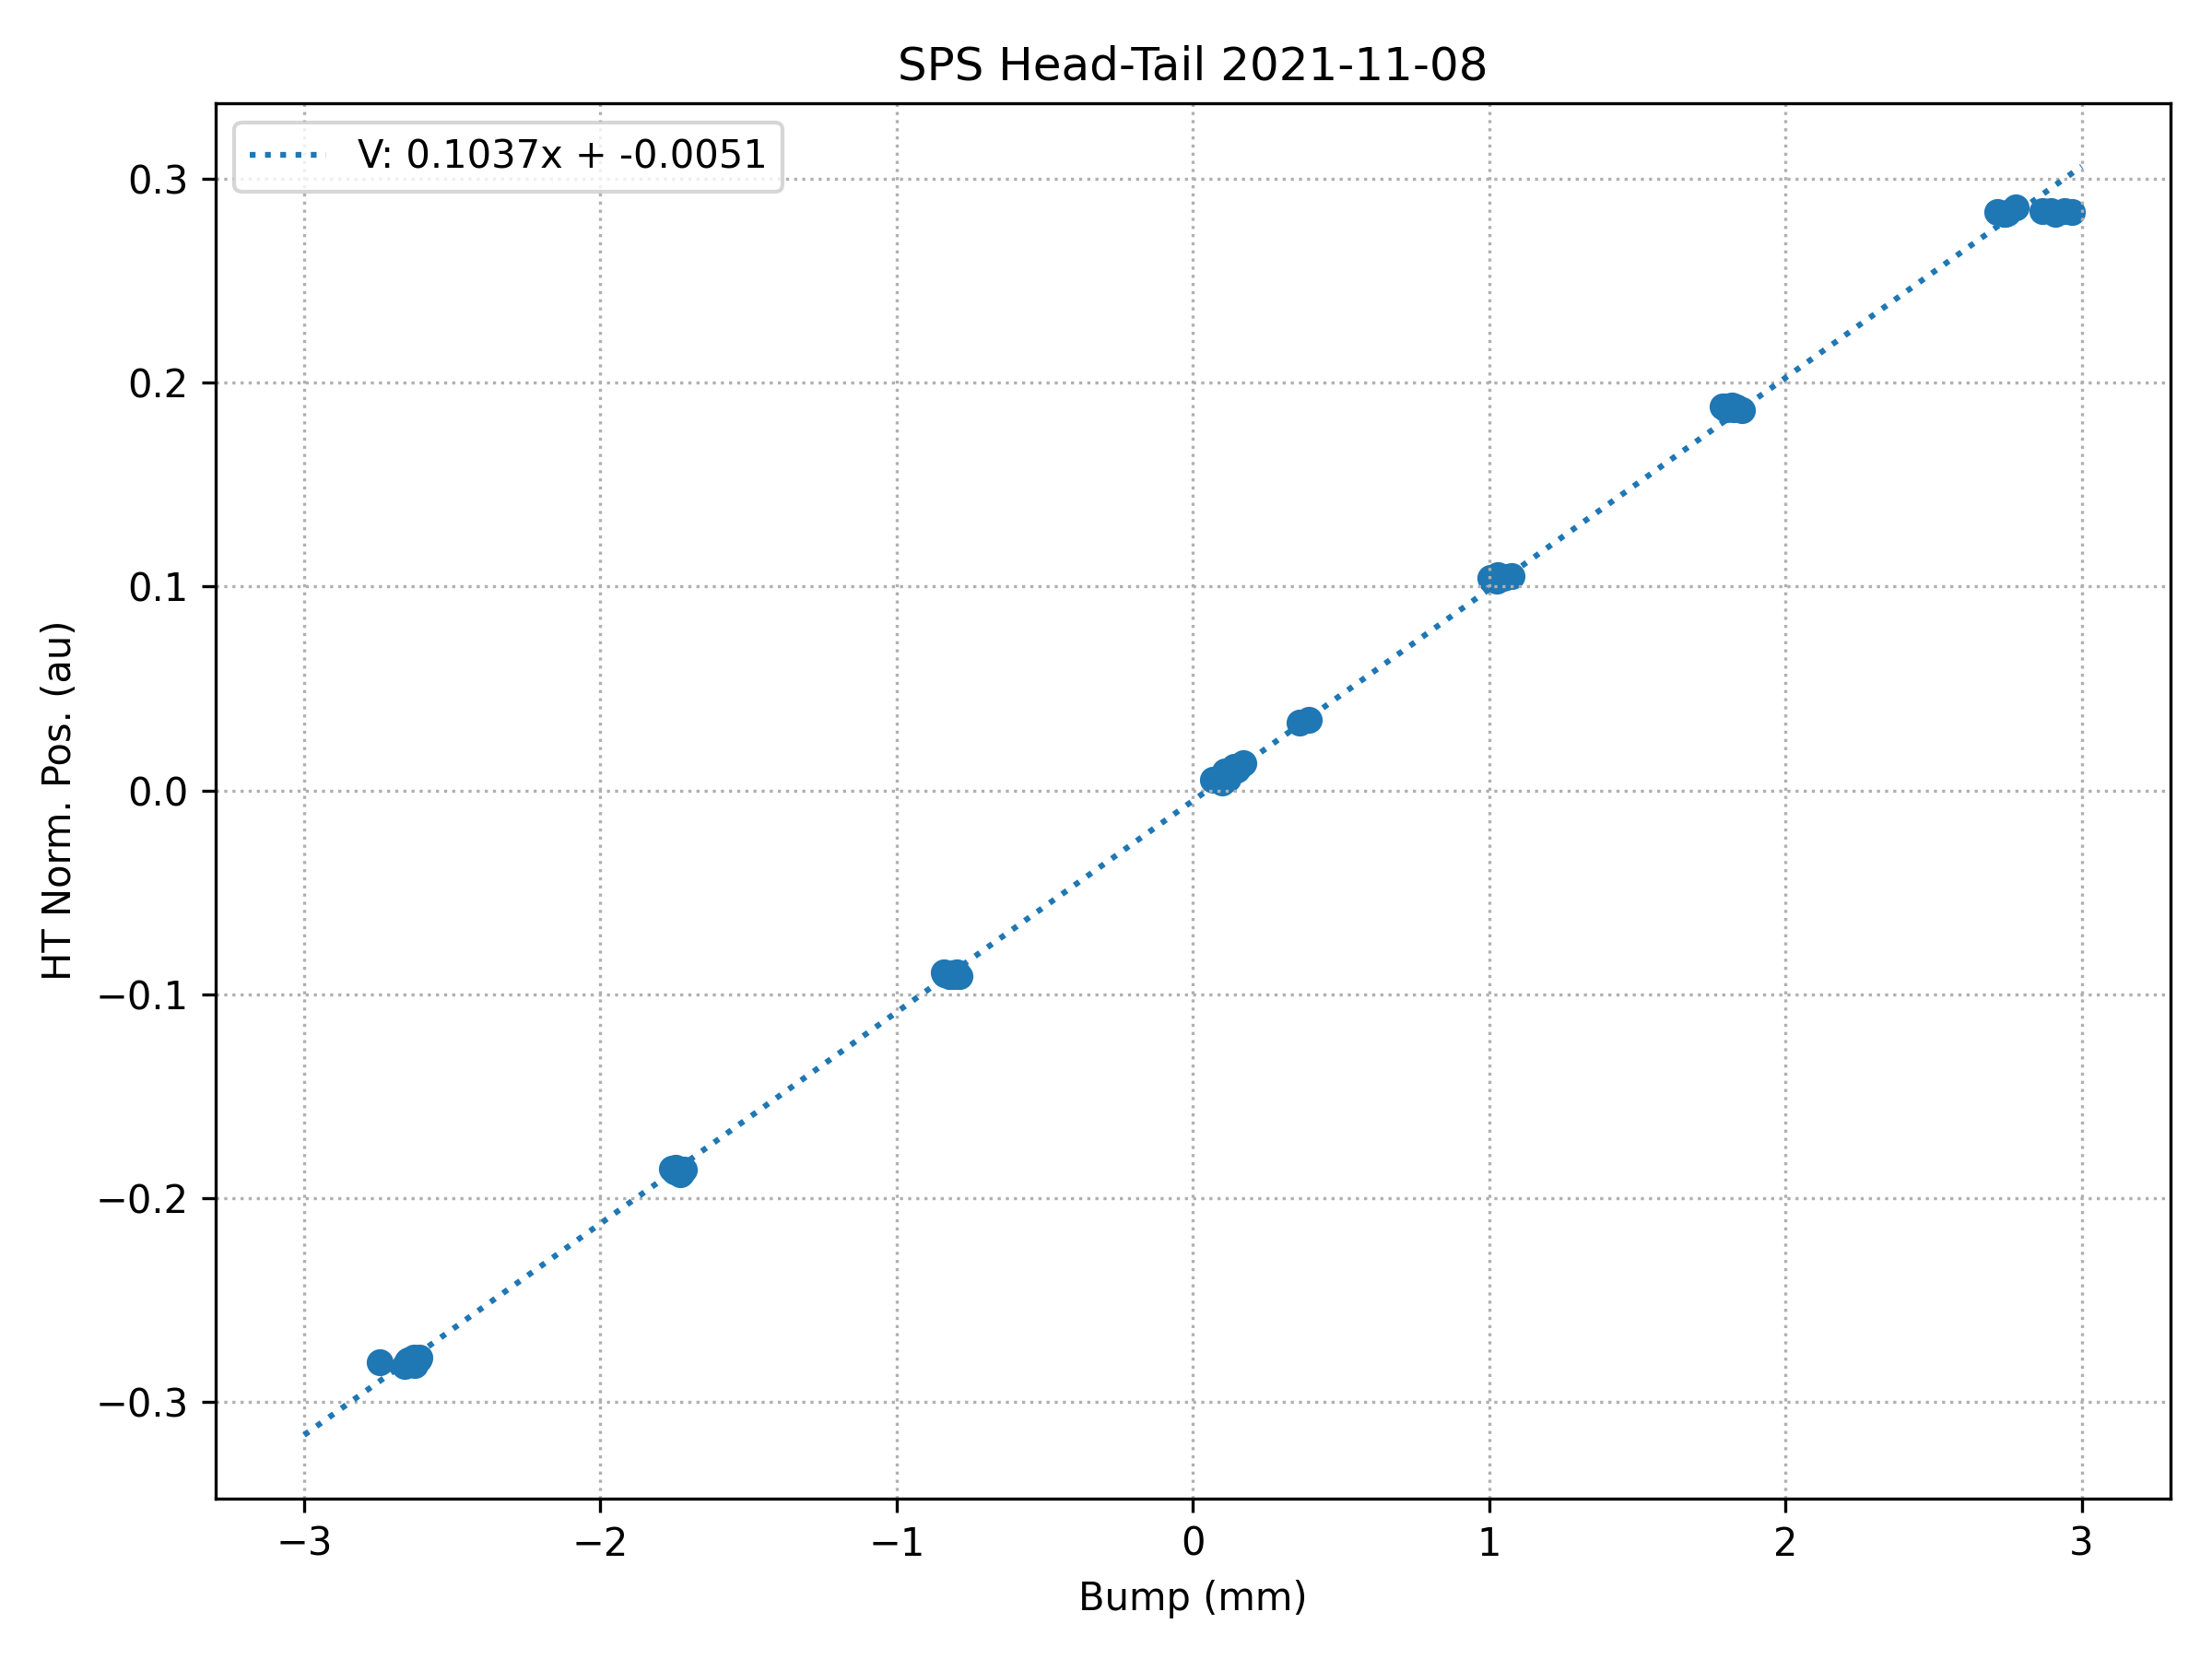
\includegraphics[width=0.7\textwidth]{images/Ch8/HT_monitor_calibration_2022.png}
        \caption{The calibration was performed by T.~Levens by performing orbit bumps (around the reference orbit) and measuring the normalised position of the bunch in the vertical plane (plane of interest). The normalised position is obtained as the difference of the signal divided by the sum. More details on the calibration procedure are given in Ref.~\cite{PhysRevAccelBeams.22.112803}. This plot is a courtesy of T.~Levens .}
        \label{fig:HT_calibration_2022_levens}
 \end{figure}


\subsection{Experiment preparation and procedure}\label{sec:cc_md_2022_preparation}
\textbf{Objectives}\\
The available machine time ($\sim$ 10 hours) for the $\CC$ experiment of 2022 was split into two parts. For the first part, the objective was to measure the emittance growth with the same noise levels and conditions as in 2018 in order a) to reproduce the observed scaling of emittance growth (see Fig.~\ref{fig:MD5_summary_plot}) and b) to benchmark the expected suppression factor from PyHEADTAIL simulations with the impedance model. This will be referred to as $\CC$ Experiment A in the following.

The objective of the second part was to investigate the effects of impedance and amplitude detuning on the emittance growth from $\CC$ phase noise. The preceding analysis of the PyHEADTAIL simulations revealed a significant sensitivity of the emittance growth suppression on amplitude-dependent tune shift (e.g. Fig.~\ref{fig:MD_2018_impedance_simulations}). This behavior can be tested experimentally in the SPS with the use of the Landau octupole families, which allow for the introduction of controlled detuning with amplitude. A successful reproduction of this behavior would provide the proof-of-concept for the emittance growth suppression mechanism from the beam transverse impedance. This will be referred to as $\CC$ Experiment B in the following. It should be mentioned, that for this experiment the octupoles of the LOD family are employed as they mostly in the vertical plane which is the plane of interest in this studies (vertical $\CC$ module which results to vertical emittance growth).

\textbf{Preparational studies with PyHEADTAIL simulations}\\
In preparation for the $\CC$ experiments (A and B) the emittance growth in the presence of $\CC$ RF phase noise was simulated with PyHEADTAIL including the most up-to-date SPS impedance model~\cite{updated_sps_wakfields_model} as a function of different octupole strengths, $k_{\mathrm{LOD}}$. The beam and machine parameters are the ones reported in Table~\ref{tab:machine_beam_param_2022} which correspond to the experimental conditions of 2022. The emittance growth is induced by $\CC$ RF phase noise with a power spectral density of 1.68\,$\mathrm{rad^2/Hz}$ in the first betatron sideband which results in about 25\,nm/s. It should be highlighted that this noise level is much stronger than the levels of the injected artificial noise used in the experiment, in order to have nice observables in the simulation time of just 2.5\,s. Therefore, the goal of the experiments was to reproduce the simulated suppression factor and behavior only and not the exact numbers. Last, the simulation setup and the $\CC$ RF phase noise were simulated as discussed in Chapter~\ref{Ch:suppression_impedance}. 

The emittance growth was simulated over a range of twenty one $k_\mathrm{LOD}$ values equally spaced from -28.2\,$\mathrm{1/m^4}$ to +28.3\,$\mathrm{1/m^4}$. Nevertheless, in the simulations, no actual octupolar elements were used in order to avoid the excitation of resonances as discussed in Section~\ref{sec:first_obs_suppression}. Instead, following the preceding PyHEADTAIL simulations, the effect of LODs is introduced as a change in the phase advance of the individual particles depending on their individual actions and defined by the corresponding detuning coefficients. The study was performed for zero horizontal detuning coefficient, $\alpha_{\mathrm{xx}}$=0 while the values of the vertical, $\alpha_{\mathrm{yy}}$, and the cross-term, $\alpha_{\mathrm{yx}}$, coefficients were estimated using MAD-X~\cite{madx}.

Figure~\ref{fig:pyheadtail_cc_impedance_2022_md_octupole_current} illustrates the dependence of the $\CC$ RF phase noise-induced emittance growth on the LOD strength, in the absence (blue) and the presence (orange) of the wakefields. The analytical prediction of the model of T.~Mastoridis and P.~Baudrenghien is also given to facilitate the identification of the suppression factor from the impedance (horizontal black dashed line). As usual, in the absence of wakefields, there is a very good agreement between the simulation results and the theoretical predictions. In the presence of wakefields, the expected dependence on the tune spread appears. The rms tune spread values in the secondary horizontal axis, are computed using both the $\alpha_{\mathrm{yy}}$ and $\alpha_{\mathrm{yx}}$ coefficients using Eq.~\eqref{eq:rms_amplitute_detuning_3}.

% 1) Slides on computing the octupole current: https://docs.google.com/presentation/d/1VgGMqCevej4Eh7bjdGFSEPVI0zLxqB2S5FxLtFGhp2I/edit#slide=id.ge970b2a80a_0_16
The green and yellow areas indicate regimes where the octupoles require less than 200\,A and 400\,A respectively for their operation. The maximum operational current for the LODs in SPS is 400\,A. However, due to their planned continuous operation in multiple coasts, the LOD current should stay below 200\,A. The required current for the octupoles is computed from their strength, $k_\mathrm{LOD}$, using Eq.~\eqref{eq:I_vs_B3_relation_lof}


% /eos/user/n/natriant/pyheadtail_data/final_for_thesis/2022_conditions/CC1/deyRates_sps_270GeV_PN1e-8_400MHz_SPS_CC2_updatedWakes_y-plane_WakesOFF_vs_WakesON_new_QpxQpy0.5_6D_Nb5e5_intensity3e10Scan_vs_TuneSpreadvsExpectedSPS_octupole_current.png
\begin{figure}[!h] % Email communication with T. Levens on 8 November 2021.
   \centering         
   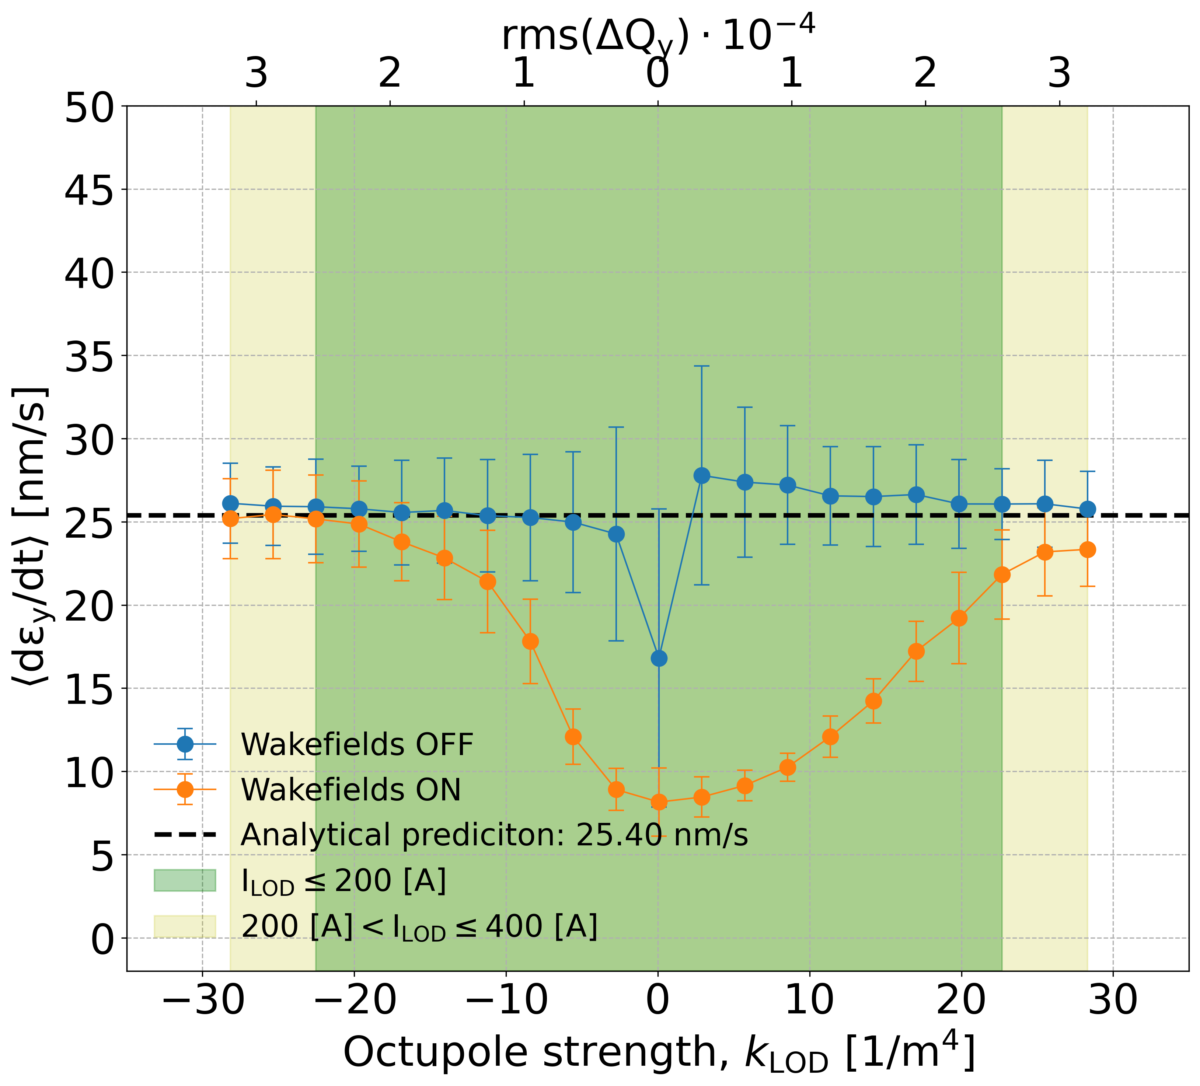
\includegraphics[width=0.8\textwidth]{images/Ch8/deyRates_sps_270GeV_PN1e-8_400MHz_SPS_NewWakesAllcontributions_appendWakes_y-plane_WakesONvsOFF_QpxQpy1_6D_Nb5e5_intensity3e10Scan_vs_TuneSpreadvsExpectedSPS_octupole_current.png}
       \caption{Transvserse emittance growth driven by CC RF phase noise without (blue) and with (orange) the imepdance effects. The green and yellow areas indicate regimes where the octupoles require less than 200\,A and 400\,A respectively for their operation.}
       \label{fig:pyheadtail_cc_impedance_2022_md_octupole_current}
\end{figure}

Looking at the Fig.~\ref{fig:pyheadtail_cc_impedance_2022_md_octupole_current} the following observations are made:
\begin{enumerate}
   \item The asymmetry on the suppression factor for positive and negative detuning with amplitude observed in the simualtions for the 2018 experimental conditions (Chapter~\ref{Ch:suppression_impedance}) seems to be mitigated here. Nevertheless, in order to exit the suppression region the negative polarity of the octupoles (LOD) should be preferred.
   \item Without powering the octupoles (2018 conditions), $k_\mathrm{LOD}$=0, a suppression of a factor of about 3 is observed.
   \item Even for the strongest octupole strengths, $| k_\mathrm{LOD} |\approx 30 \ \mathrm{1/m^4}$, the required current remains below 400\,A. Consequently, no crucial limitations are introduced to the experiment from the octupoles operation.
\end{enumerate}

\textbf{Steps}\\
The experiment took place on 16th of May of year 2022 and as a given a total time window of about 10 hours (start: $\sim$ 9:15 , end $\sim$18:40). The steps taken during the experimental study were the following:

\begin{enumerate}
   \item Calibration of the voltage and phase offset of the CC.
   \item Measurement of the background growth rate in coast: CC is switched on but with no additional noise injected in its RF system and the Landau octupoles switched OFF.
   \item Measurement of the emittance growth with the Landau octupoles switched OFF and for four different noise levels as in 2018 (CC Expereiment A). For each noise level a new bunch was injected.
   \item Measurement of the emittance growth for a selected noise level and varying octupole strength (CC Expereiment B). For each octupole setting a new bunch was injected in the SPS.
\end{enumerate}


The details and the results of the above mentioned steps will be presented in the following subsections.

\subsection{Calibration of CC voltage and phase offset}\label{subsec:cc_calibration_2022}
The first step in the CC experiment was to calibrate its voltage and phase offset. The calibration took place following the procedure described in Section... at 270\,GeV and it lasted for about 15 minutes (start: $\sim$ 9:40, end: $\sim$09:52).

To provide an overview, the calibration was performed by varying the inspector phase of CC1 from -180 to + 180 degrees in steps of 30 degrees. For each step, the crabbing signal was acquired with the HT monitor and the CC voltage signal was reconstructed. For each acquisition, the $\CC$ voltage at the center of the bunch, $t=0$, was plotted as a function of the corresponding inspector phase. The results of the inspector phase scan for $\CC$1 are summarised in Fig.~\ref{fig:Vcc_calibration_md_2022}.

\begin{figure}[!h] % /eos/user/n/natriant/2022/SPS_MDs_2022/cc_md_16May2022/HT_monitor_phase_CC_offset_calibration
   \centering         
   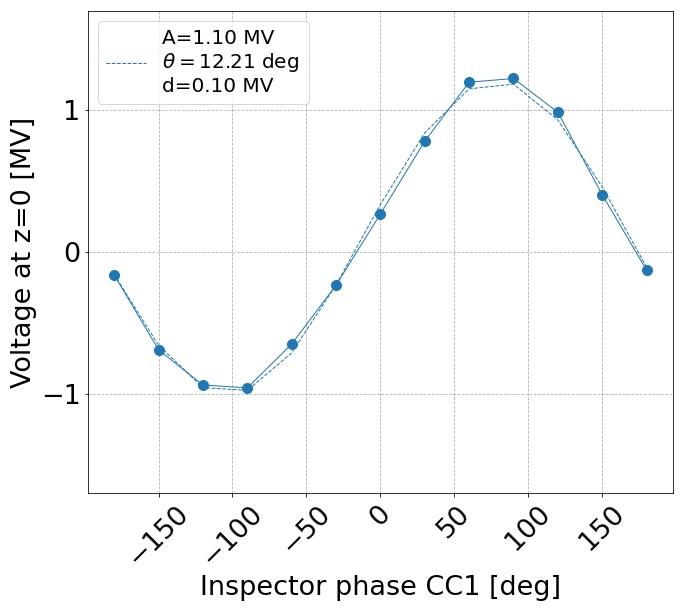
\includegraphics[width=0.7\textwidth]{images/Ch8/Vcc_at_z_zero_vs_inspector_phase_CC1_for_thesis.png}
       \caption{Calibration plot for the CC1 as obtained during the experiment on 16th of May 2022, displaying the CC voltage at the center of the cavity $t=0$ for different values of the inspector phase.}
       \label{fig:Vcc_calibration_md_2022}
\end{figure}

From the beam based measurements with the HT monitor the voltage of CC1 was found to be 1.1\,MV very close to the targeted one (1\,MV). The phase offset was found to be 12.21 degrees. For the rest of the experiment, inspector phase was set to the opposite of the phase offset such as the CC phase is zero.

Between $\sim$11:39 and $\sim$11:45 the same scan for CC2 was attempted. However, the cavity tripped systematically due to issues associated with the change of the RF phase. Treating it would have been time-consuming which was not an option due to the very limited machine time of the MD. Therefore, for the measurements in 2022 $\CC$1 was used.
% CC2 tripped: see the entry of the logbook 4/5/2022, at 11:30:30 

\subsection{Measurement of background growth rate in coast}\label{subsec:measured_background_growth_cc_md_2022}
After the calibration of the CC1, the coast at 270\,GeV was set up for the emittance growth measurements. First, the background emittance growth, with no additional noise injected in the CC and the Landau octupoles switched off was measured. The background emittance growth was found to be similar in both transverse planes and in particular $d\epsilon_x /dt$ = 0.81\,$\mathrm{\mu m}$ and $d\epsilon_y /dt$ = 0.84\,$\mathrm{\mu m}$ in the horizontal and vertical planes respectively. This measured background emittance growth is illustrated in Fig~\ref{fig:cc_md_2022_background_growth_in_scan} for both the horizontal (blue) and vertical (red) planes.

\begin{figure}[!h] % /eos/user/n/natriant/2022/SPS_MDs_2022/cc_md_16May2022/roundA_online_analysis_ws/online_analysis_scripts_figures/coast1
   \centering         
   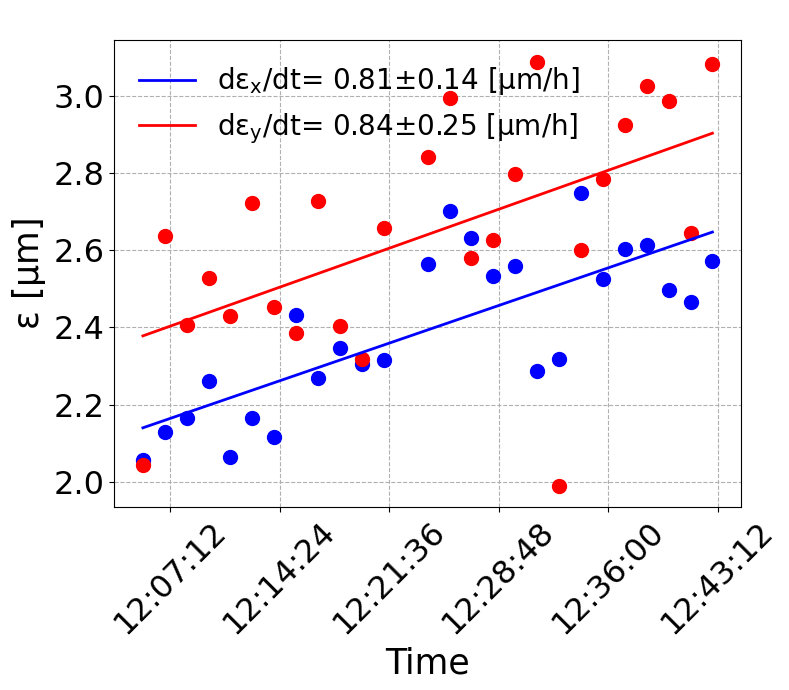
\includegraphics[width=0.7\textwidth]{images/Ch8/cc_md_2022_background_in_scan.png}
       \caption{Horizontal (blue) and vertical (red) background emittance growth measured during the experiment with CC1 in 2022, with no injected artificial noise and with the Landau octupoles switched OFF.}
       \label{fig:cc_md_2022_background_growth_in_scan}
\end{figure}
% There was no valid reason to exclude any of the points even the outliers.

The applications used in the control room for the monitoring of the SPS machine have undergone an upgrade between the years 2018 and 2022. The latest applications which activate the Wire Scanners and automatically compute the emittance values from the profiles do not compute the respective errors. Nevertheless, the profiles' data are available and thus the uncertainties of the emittance values can be calculated at a later post-processing stage. This post-processing showed that the uncertainties of the emittance values (computed as shown in Chapter~\ref{Ch:2018_analyisis}) are 2-3 orders of magnitude smaller than the emittance values themselves \footnote{See Appendix~\ref{sec:sps_transverse_beam_profiles}}. Therefore, their impact is insignificant and the uncertainties of the emittance growth rates are dominated by the fluctuation of the Wire Scanner acquisitions. To this end, they are not shown in the emittance growth plot nor included in the fit to facilitate the analysis.

From the above figure, it is evident that there is a significant fluctuation in the emittance values in both transverse planes. By looking at the beam profiles, no evidence (e.g. corrupted profiles, abnormal tails, large errors on the gaussian fit results) was found to exclude some of the points. This fluctuation is introduced by the Wire Scanners used for the measurements. As discussed with the experts it appears to be within the limitations of the instrument for these small emittance values. In order to reduce the sensitivity of the linear fit (from which the emittance growth rates are obtained) longer measurements are required (at least 40 minutes). For larger emittance growth rates, or in other words for larger emittance values, these fluctuations are mitigated. The individual measurements from the different coasts during the experiment can be found in the Appendix...

Finally, for reference, the "natural" amplitude and phase noise at 8\,kHz were measured to be -130.2\,dBc/Hz and 125.7\,dBc/Hz respectively. The theoretically~\cite{PhysRevSTAB.18.101001} expected emittance growth from those noise levels was 0.05\,$\mathrm{\mu/h}$ and 0.19\,$\mathrm{\mu/h}$ in the horizontal and vertical planes respectively from both noise types combined.
% y-plane --> AN: 0.045 um/h, PN: 0.14 um/h
% x-plane --> AN: 0.002 um/h, PN: 0.05 um/h
% Directory to compute these rates: /afs/cern.ch/work/n/natriant/public/SPS_MDs_2022/cc_md_16May2022/cmpt_emit_growth_theoretical_model
% Also some of the growth in the horizontal plane is expected by the IBS. How much I do not know yet.
The rest of the observed growth rates, is due to other sources which are not yet will identified (see discussion in Chapter~\ref{Ch:2018_analyisis}).

\subsection{Results of CC Experiment A: scaling of emittance growth with noise power}

The objective of the first part of the experiment was to reproduce the scaling of the emittance growth driven by CC RF noise with the noise power as observed in 2018. Four different levels of artificial noise were injected in the RF system of the $\CC$ as listed in Table~\ref{tab:noise_settings_2022} and the emittance evolution was recorded in coast every $\sim$1.5 minute. For each noise level, a new bunch was injected such as all the measurements took place with the same initial conditions. The duration of each coast varied from about 30 minutes for the low noise levels to about 20 minutes for the strong noise. The 

For the strong noise, less measurement time is sufficient since the growth rate obtained from the linear fit on the emittance values is not sensitive to the fluctuations due to the Wire Scanner. Additionally, for strong noise, the emittance reaches very quickly very large values, about 8-10\,$\mathrm{\mu m}$, which eventually degrades the quality of the beam.

Figure~\ref{fig:cc_md_2022_overview_plots_noise_scan} illustrates the transverse emittance growth measured in the SPS in 2022 for the four different noise levels injected in the $\CC$ RF system increasing from top left to bottom right. It can be seen, that there is a clear emittance growth in the vertical plane which is faster for stronger noise as expected. A growth in the horizontal emittance is also observed it seems independent from the growth in the vertical. This is also confirmed in Fig.~\ref{fig:H_V_emit_growth_noise_scan} where the vertical and horizontal growth rates are plotted as a function of the four different phase noise levels. Consequently, in the following analysis of the experimental data the growth in two planes will be treated independently (unlike in 2018, see Chapter~\ref{Ch:2018_analyisis}.)\textcolor{red}{These last sentences need to be modifief after checking again the 2018 data to see if there was indeed coupling or not.}


% Note 1, figures: /eos/user/n/natriant/2022/SPS_MDs_2022/cc_md_16May2022/roundA_online_analysis_ws/for_thesis
% Note 2, scripts to plot: /afs/cern.ch/work/n/natriant/public/SPS_MDs_2022/cc_md_16May2022/ws_measurements 
\begin{figure}[htp]
   \centering
   \begin{subfigure}{.45\textwidth}
       \centering
       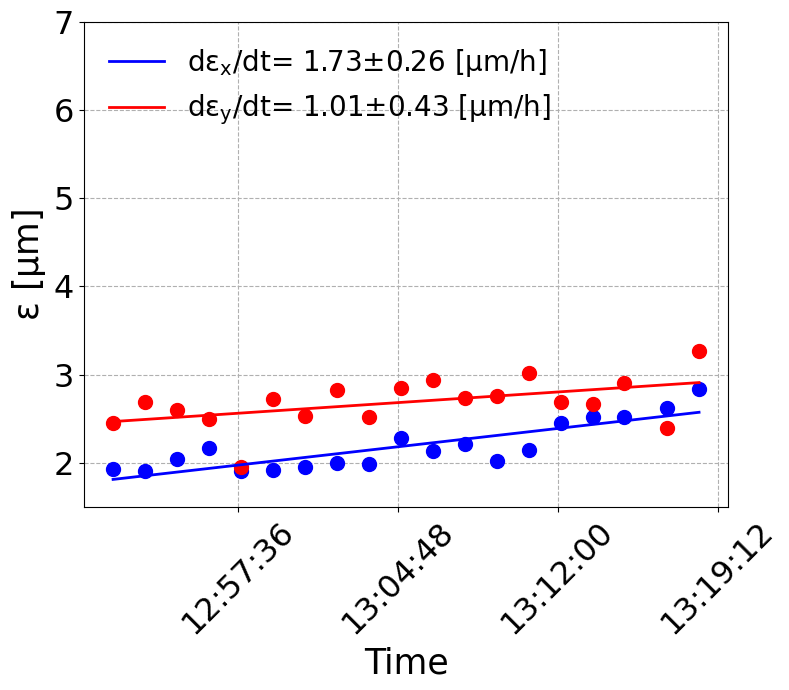
\includegraphics[width=.95\linewidth]{images/Ch8/emit_vs_time_Set1_coast2.png}  
       \caption{-115.2\,dBc/Hz}
       \label{fig:cc_md_2022_coast2}
   \end{subfigure}
   \begin{subfigure}{.45\textwidth}
       \centering
       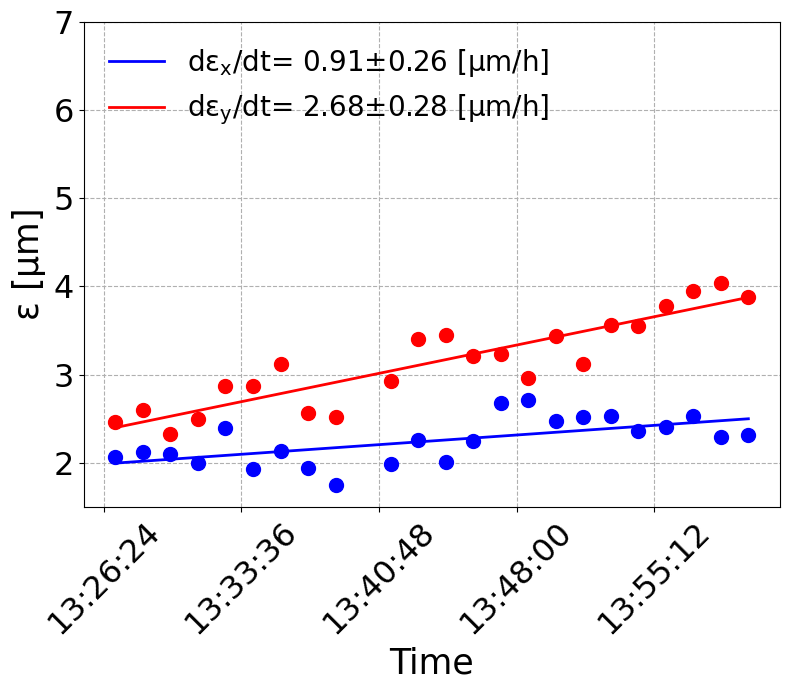
\includegraphics[width=.95\linewidth]{images/Ch8/emit_vs_time_Set1_coast3.png}  
       \caption{-109.5\,dBc/Hz}
       \label{fig:cc_md_2022_coast3}
   \end{subfigure}
   \begin{subfigure}{.45\textwidth}
       \centering
       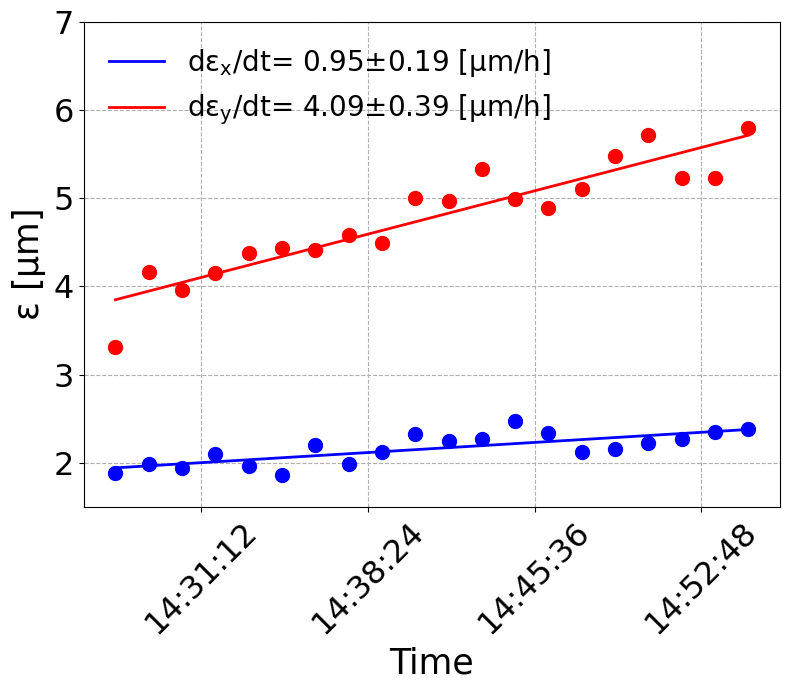
\includegraphics[width=.95\linewidth]{images/Ch8/emit_vs_time_Set1_coast4.png}  
       \caption{-104.7\,dBc/Hz}
       \label{fig:cc_md_2022_coast4}
   \end{subfigure}
   \begin{subfigure}{.45\textwidth}
           \centering
           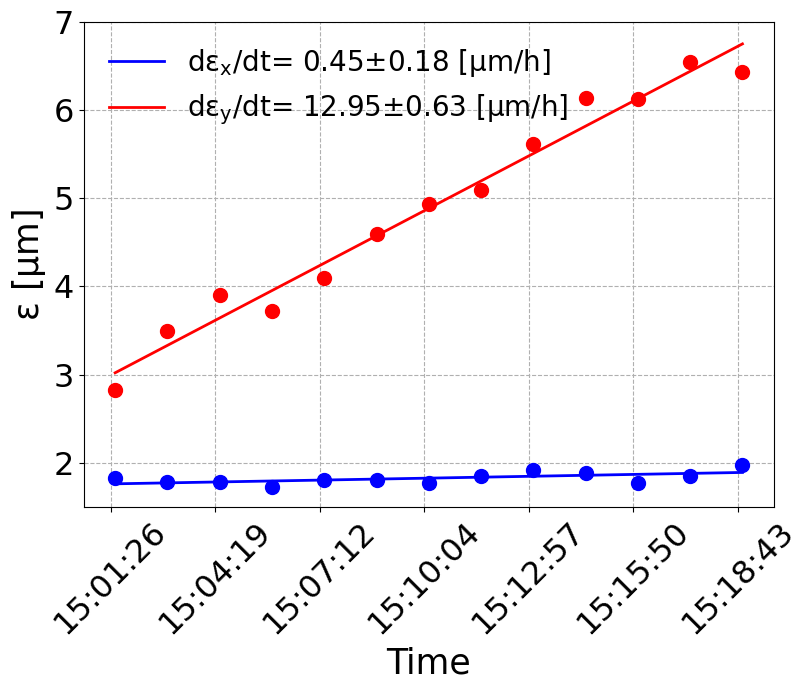
\includegraphics[width=.95\linewidth]{images/Ch8/emit_vs_time_Set1_coast5.png}  
           \caption{-100.1\,dBc/Hz}
           \label{fig:cc_md_2022_coast5}
   \end{subfigure}
   \caption{Horizontal (blue) and vertical (red) emittance evolution of a single bunch during the CC experiment on May 16, 2022. The different phase noise levels injected in the RF system of CC1, are displayed at the captions of each plot.}
   \label{fig:cc_md_2022_overview_plots_noise_scan}
\end{figure}

% Figure: /eos/user/n/natriant/2022/SPS_MDs_2022/cc_md_16May2022/roundA_online_analysis_ws/summary_plots/for_thesis/emit_H_and_V_noise_scan.png
\begin{figure}[!h] 
     \centering         
   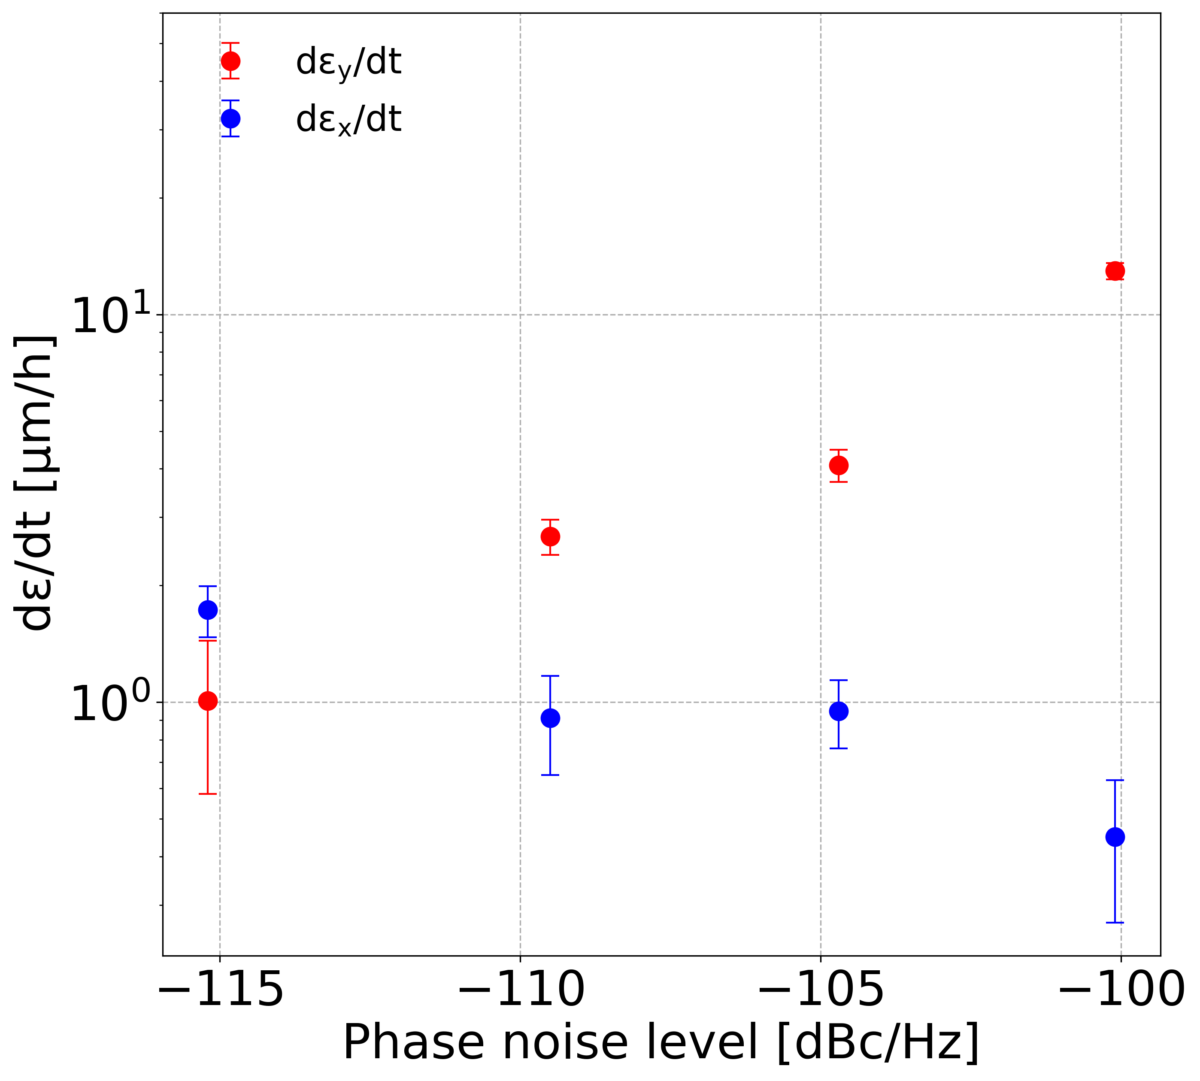
\includegraphics[width=0.7\textwidth]{images/Ch8/emit_H_and_V_noise_scan.png}
       \caption{Overiview plot of the emittance growth study with noise injected in the CC1 in 2022. The measured horizontal (blue) and vertical (red) emittance growth rates are shown as a function of the different phase noise levels of applied noise. The error bars indicate the error of the linear fit on the emittance values (see Section~\ref{sec:emit_growth_meas_2018}).}
       \label{fig:H_V_emit_growth_noise_scan}
\end{figure}


\textbf{Summary plot}\\
Figure~\ref{fig:V_emit_growth_background_subtracted_noise_scan} compares the measured (red) and the theoretically calculated (black) vertical emittance growth rates for the different phase noise levels. For the comparison the background growth rate measured in the vertical plane (see Section~\ref{subsec:measured_background_growth_cc_md_2022}) of 0.84\,$\mathrm{\mu m /h}$ is subtracted from the measured values. The theoretically calculated values are obtained inserting the phase noise levels of Table~\ref{tab:noise_settings_2022} in Eq.~\eqref{eq:dey_pn} for rms bunch length of $4 \sigma_t$ = 1.83\,ns, energy of 270\,GeV and the vertical beta function at the location of CC1, 76.07\,m . The subtraction of the background has practically no impact on the high noise levels but it is significant for the small ones.

% Figure: /eos/user/n/natriant/2022/SPS_MDs_2022/cc_md_16May2022/roundA_online_analysis_ws/summary_plots/for_thesis/emit_V_background_subtracted_noise_scan.png
\begin{figure}[!h]
   \centering         
   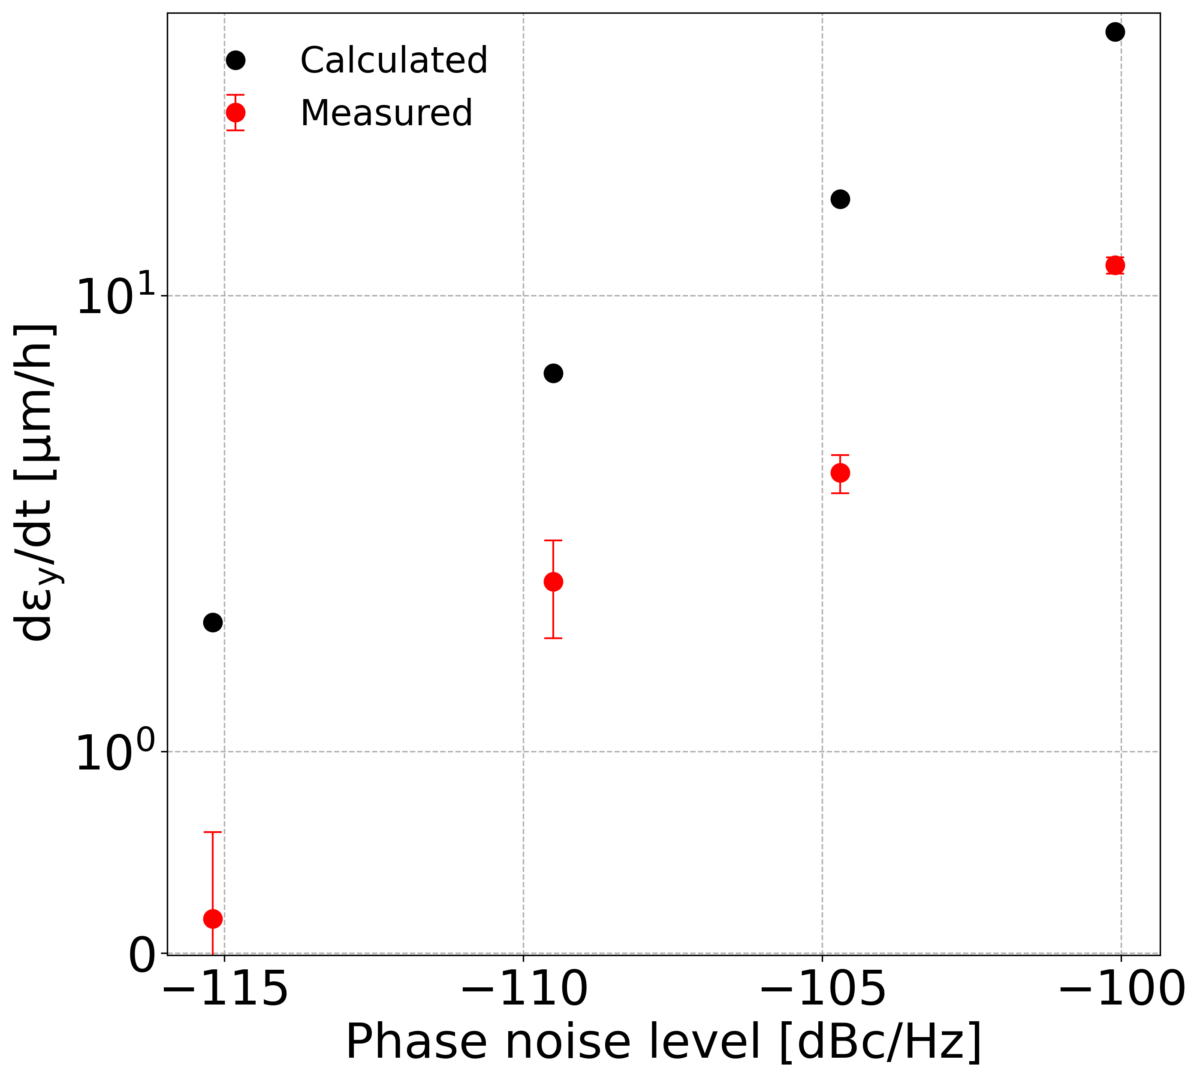
\includegraphics[width=0.7\textwidth]{images/Ch8/emit_V_background_subtracted_noise_scan.png}
       \caption{Summary plot of the emittance growth study with different noise levels injected in the RF system of CC1 in 2022. The vertical measured growth rate (red) and the expected growths from the theoretical model~\cite{PhysRevSTAB.18.101001} (black) are shown as a function of the different levels of applied phase noise. The error bars indicate the error of the linear fit on the emittance values (see Section~\ref{sec:emit_growth_meas_2018})}
       \label{fig:V_emit_growth_background_subtracted_noise_scan}
\end{figure}

From Fig.~\ref{fig:V_emit_growth_background_subtracted_noise_scan} it becomes evident that the theory systematically overestimates the measured growth rates. The averaged discrepancy over all noise levels, but the first one, is a factor 4: numerical values are given in Table...



\begin{table}[!hbt]
	\centering
   \caption{Comparison between the measured and the calculated transverse emittance growth rates for the different phase noise levels during the CC experiment of 2022. The analytical emittance growth rates were computed using Eq.~\eqref{eq:dey_pn} for rms bunch length of $4\sigma_t$=1.83\,ns.}
	\begin{tabu} to \textwidth { X[c,m] X[c,m] X[c,m] }
		&& \\[-6mm]
		\toprule \toprule
		\multicolumn{1}{c}{$\mathbf{10\,\boldsymbol{\log}_{10} \mathcal{L}(f)}$} &
      \multicolumn{2}{c}{\textbf{Growth rate [}$\mathbf{\boldsymbol{\mu}}$\textbf{m/h]}}  \\
		%\bottomrule
      \multicolumn{1}{c}{\textbf{[dBc/Hz]}} & \multicolumn{1}{c}{\textbf{\textbf{Measured}}} & \multicolumn{1}{c}{\textbf{Calculated}}  \\
      \midrule
      \multicolumn{1}{c}{-115.2}  & \multicolumn{1}{c}{1.05} & \multicolumn{1}{c}{0.44} \\
      
      \multicolumn{1}{c}{-109.5}  & \multicolumn{1}{c}{1.10} & \multicolumn{1}{c}{1.18} \\

      \multicolumn{1}{c}{-104.7}  & \multicolumn{1}{c}{1.03} & \multicolumn{1}{c}{1.28}  \\

      \multicolumn{1}{c}{-100.1}  & \multicolumn{1}{c}{1.06} & \multicolumn{1}{c}{2.28}  \\ 
      \arrayrulecolor{black}\bottomrule
	\end{tabu}
   \label{tab:MD5_bunch1_results}
\end{table}


This is in agreement with the experimental observations of 2018 (see Fig.~\ref{fig:MD5_bunch1_theory_vs_meas})


\subsection{Results of CC Experiment B: sensitivity to amplitude-dependent tune shift} 

\section{Experiment with beam damper as noise source}



\newpage

\section{Strategy and preparational studies}\label{sec:strategy_md_2022}
% MD planning: https://docs.google.com/presentation/d/13b4KAywwANL_hk0ttAmxjW8P0zLzrJpNUKiEGYtgD3w/edit#slide=id.p 
The experiment of 2022, was consisted of emittance growth measurements at 270\,GeV in coast mode, as in 2018. 

The objective of the second part was to investigate the effects of impedance and amplitude detuning on the emittance growth from $\CC$ phase noise. The preceding analysis of the PyHEADTAIL simulations revealed a significant sensitivity of the emittance growth suppression on amplitude-dependent tune shift (e.g. Fig.~\ref{fig:MD_2018_impedance_simulations}). This behavior can be tested experimentally in the SPS with the use of the Landau octupole families, which allow to introduce controlled detuning with amplitude. A successfully reproduction of this behavior would provide the proof-of-concept for the emittance growth suppression mechanism from the beam transverse impedance.




Tonise oti to behavior einai auto pou thes na kaneis reproduce oxi ta exact numbers. des parousiasi high schooll.


In particular, the LOD family was used which affects primarly the vertical plane. The reason behind this, is that as in 2018, in the experiment of 2022 the DQW $\CC$ module was used which provides a vertical deflection of on the beam and hence the focus was put in the vertical plane.


\subsection{extra}
check the amplitude detuning with ampltidue
h%ttps://docs.google.com/presentation/d/1yaGKJ20O-jVg0R3bdj62l5VzltwjBBHtphKq5HI9xrY/edit#slide=id.g104dd3ff735_0_184


\section{Simple model of Xavier vs experimental results}
for dipolar nosie


The Landau octupoles current might be a limtiing factor.


If you want to describe the steps for the MD see section 3.3 David amorim.